\chapter{Introduction}
Crystallisation is one of the oldest forms of phase separation 
used by humanity\cite{Schoen1956}, put simply, it is the 
formation and growth of a new structured phase within 
a disordered bulk phase. This has applications in a 
number of industries such as pharmaceuticals, food 
production, and electronics \cite{Myerson2002}; where 
the extraction of dilute materials can help improve 
product quality while keeping production costs low. 
The industrialisation of crystallisation has allowed 
engineers to reliably and efficiently induce the crystal 
formation within a bulk phase. However, while on a 
large scale crystallisation is seemingly an understood 
physical process, just a small amount of investigation 
into the literature reveals that at a micro scale there 
is yet to be unifying theory that can accurately explain 
the process of crystallisation \cite{Fu2021}. Of which 
there two primary areas of focus, nucleation and crystal 
growth. The latter focusing on how an already stable 
crystal grows and how it takes on its final shape; 
whereas the former is more concerned with which factors 
contribute to its formation in order to control crystal growth.

The focus of this research is partly based around investigating
the impact of a focused electromagnetic field can influence the 
nucleation process by inducing shear flow within the bulk phase. 
This in hope that the localised EM field can be used to study 
different phenomena in nucleation in order to develop a better
understanding of the underlying mechanisms.

\section{Nucleation}
Nucleation is an example of a binary phase separation, 
where a dilute phase is miscible in a bulk phase, more 
often called the solute and solvent respectively. Because 
of thermodynamics, the two can only remain in equilibrium while 
below a specific concentration ($C_{eq}$) - below which 
the chemical potential $\mu$ for a miscible solution 
is greater than the potential required to separate 
the two phases. Once $C_{eq}$ is exceeded there is a chemical
 potential difference driving the solution to separate the 
two phases. Since different combinations of solute and solvent
will have different equilibrium concentrations, researchers often 
instead measure the ratio between the solute and solvent by using 
'supersaturation', one form of measuring supersaturation is shown 
below \cite{Mullin2001}:
\begin{align}
	\label{eq:supersaturation}
	S(T) = \frac{C_{sol}}{C_{eq}(T)}
\end{align}
Where $C_{sol}$ is just the solute concentration, $C_{eq}(T)$
is the equilibrium concentration at temperature $T$.
While the solution remains supersaturated there is a 
chemical potential driving force for the solute 
to coalesce and separate from the solution as an ordered solid, 
the first formation of the crystal is referred to as the 
nucleus and understanding its formation of has been the 
focus of researchers for decades now. Typically, for an 
industrial crystallisation process the working principle 
is based on controlling and manipulating the supersaturation
of the system. 

\subsection{Primary vs Secondary nucleation}
From an industrial perspective, the nucleation process can
be broadly categorised into either primary of secondary 
nucleation. The former being described as the formation of an
initial nucleus within the bulk phase; absent of any external
stimuli primary nucleation is considered stochastic and is typically
undesirable for industrial applications where short and consistent 
residence times are desirable. At a small scale one can estimate the 
nucleation rate by making repeated measurements of sample solutions 
and seeing how many have nucleated after a given time, giving us a 
Poisson distribution.

\begin{align}
	P(t) = 1 - exp\left[-JV(t-t_g)\right] = \frac{M^*(t)}{M}
\end{align}

Where $J$ is the nucleation rate, $t_g$ is the 'growth time', $V$
is the volume of the individual samples, and $M^*(t)$ \& $M$ are the 
number of nucleated samples and the total number of samples used respectively.
While this is useful for studying the effects of different parameters
at a small scale, for industrial applications there are so many
additional factors at play that can throw off this estimation.

In contrast, secondary nucleation is the result of a initial 
seed crystal inducing further nucleation within the bulk solution
\cite{Botsaris1976}, in absence of a seed crystal nucleation is
near impossible. The research of Secondary Nucleation is fascinating
for its own merits; is it speculated that the supersaturation 
barrier is non-existent \cite{Cashmore2022}, and furthermore there 
are a multitude of mechanisms that can induce secondary 
nucleation making it imperative that researchers can control the
nucleation rate at an industrial scale. 

\begin{figure}[h!]
	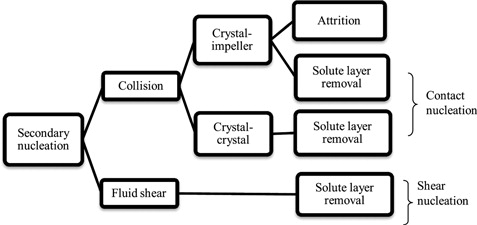
\includegraphics[width=\linewidth]{secondary_nucleation.jpg}
	\caption{Secondary Nucleation mechanisms, classified by Agrawal and Paterson \cite{Agrawal2015}}
\end{figure}

\section{Nucleation Theories}
\subsection{Classical Nucleation Theory (CNT)}
Sometimes referred to as 'Gibs Nucleation Theory' the 
original theory was first formed from the works of Volmer 
and Weber, and Frenkel \cite{Frenkel1939, Volmer1926}. 
While initially it was more focused into describing droplet 
formation in condensing vapours it was extrapolated to describe
crystallisation. The central premise of classical theory 
is that nucleation occurs stochastically throughout the bulk
phase due to collisions between individual solute molecules,
ions, or atoms; at the same time the bulk phase is resistant
to the formation of a new phase. The competition between
these random collisions and the bulk solution can be used to 
predict the probability of a newly formed nucleus.
 
Consider a supersaturated solution, after some time enough individual
sub units collide, forming a nucleus of volume $4\pi r^3/3$. 
The newly formed phase has a lower chemical potential than the 
surrounding solution, reducing the free energy of the system; 
at the same time, the formation of a new interface is resited 
by the bulk phase due to surface tension. The net free energy 
of the system for a nucleus of radius $r$ is given as \cite{Karthika2016}:
\begin{align}
	\Delta G = \frac{-4\pi r^3}{3v}k_BT\ln(S) + 4\pi r^{2}\sigma_{inf} 
\end{align}
Where $v$ is the approximate volume of an individual molecule, $k_B$
is the Boltzmann constant, and $\sigma_{inf}$ is the interfacial 
tension of the bulk solution. Plotting the free energy of the system
against nucleus size reveals a critical size above which the gain 
in free energy exceeds the interfacial tension. 
\begin{figure}[h!]
	\label{fig:free_energy}
	\centering
	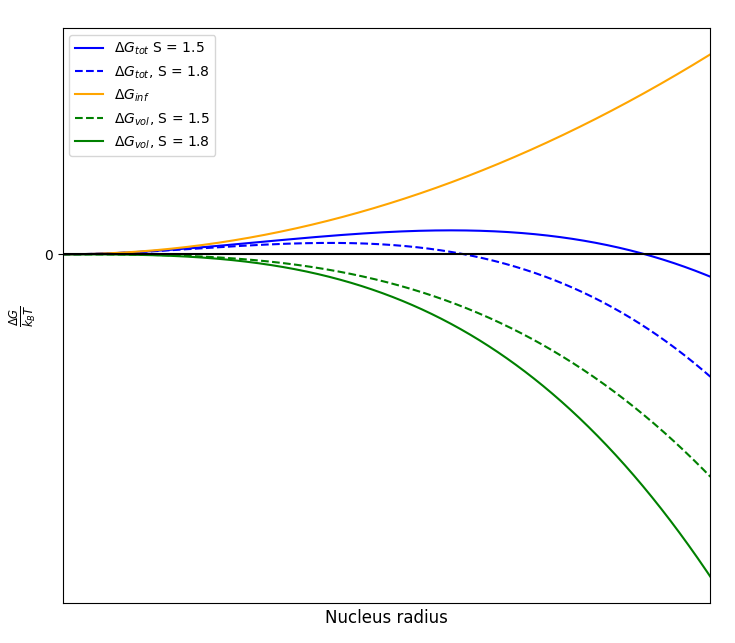
\includegraphics[width=\linewidth]{Free_Energy_Diagram.png}
	\caption{Free energy diagram of a newly formed nucleus according 
		     to the Classical Nucleation Theory. The total free energy (blue)
		     is due to the competition between the volume free energy gain
		     (green) and the interfacial free energy cost (orange). Dotted
		     lines are for a higher supersaturation than the solid lines,
		     the interfacial energy cost is independent of supersaturation.}
\end{figure}

The maximum value of $\Delta G_{tot}$ is the free energy barrier 
that any newly formed nucleus needs to overcome in order to stabilise.
The nucleation rate (the volume of new crystalline material formed per
unit time), is therefore commonly defined as being dependent on the 
energy barrier $\Delta G^*$:
\begin{align}
	J = A \ exp \left[-\frac{\Delta G^*}{k_BT} \right]
\end{align}
Where $A$ is a pre-factor that can be fine tuned to the exact demands
of the system (typically involving Zeldovich Factor, $Z$) the free 
energy barrier can be found by finding the turning point of $\Delta G_{tot}$. 

So to find the critical size $n^*$  - and therefore the nucleation rate - we simply need to know the ratio between the interfacial free energy and the volume free energy. The CNT assumes that the crystal grows is purely spherical and that the interfacial free energy is near constant (aka that of a flat surface), this assumption is not very accurate for small crystal nucleus where the changing curvature means that the surface tension varies as a function of the crystal radius. This also assumes the surrounding fluid is at rest and there are no external forces on the nucleus that might distort the shape of said nucleus; though there has been theoretical work looking into how the CNT behaves under shear flow \cite{Debuysschere2023, Mura2016, Richard2015}

Furthermore, multiple experiments have already verified that crystals can form any number of structures and can even transition through multiple structures as it grows, meaning that the interfacial tension will constantly change as the particle grows. Furthermore, because we are assuming that the surface energy is constant the pre-exponential factor that is computed from experimental data, and the factor predicted by theory often disagree with one another to several degrees of magnitude. 

There are several results that indicate that the CNT is not a good fit for nucleation rates:
\textcolor{red}{
	\begin{itemize}
		\item Discrepancy in vapor-liquid nucleation systems to the extent that CNT was off by a factor of more than 2000 \cite. 
		\item In glass formation, nucleation kinetics are incredibly important to understand as the crystallization process is not desired when producing glass. We want to cool the molten solution so that the solid does not have time to reorganize itself into an ordered structure. To understand nucleation kinetics in glass formation we need to understand that as crystals form in the glass the surface energy differs from the stable phase significantly which us poorly predicted by CNT as it assumes that crystals will have a constant structure and interaction with the bulk material [ ]. 
		\item Metal alloys can demonstrate super-cooling while not experiencing nucleation, this is because in these liquids exhibit short range dynamics which means that the liquid droplet remains unordered as it is cooled. Because CNT assumes that the droplets must be of a similar ordering to that of the bulk crystal it often struggles to consider systems where the local bond order can fluctuate between phases. [ ]
	\end{itemize}
}

CNT is often regarded as a good description of the macro system, its obvious that for all crystallization systems there is an inherent energy barrier that dictates the nucleation rate. However, for such a diverse range of possible nucleation events the CNT crudely assumes all interactions between solutes as identical; this makes it difficult to model crystallisation events using CNT without significantly modifying the model for each specific case. Recent developments in studying nucleation events have opened up new possible 'pathways' for a nucleation event to go down, by far the most common is the idea of Two step nucleation.

\subsection{Two Step Nucleation}
The two step nucleation theory is an extension to the CNT, colloid simulations showed that short range (such as in proteins \cite{Wolde1997, Gliko2005}) interactions allow for the formation of a liquid-liquid metastable phase from which a new solid phase could form \cite{Anderson2002, Karthika2016}. \textit{in situ} techniques for studying nucleation several papers reported the presence of stable liquid-like clusters that formed prior to nucleation \cite{Savage2009, Wolde1997, Soga1999}.  It can be understood by Oswald's rule \cite{Ostwald1897}, which says that any crystallising system does not 
take the path to the lowest possible energy state but instead first transitions to the state with the smallest free energy barrier, further transitions can still occur but this method minimises the overall free energy cost. If we consider the free energy diagram from before (fig.~\ref{fig:free_energy}) we can consider a case where the supersaturation is low ($S\approx1.01$) then a dense liquid droplet will have a lower chemical potential than the surrounding fluid 

\section{Crystallisation methods}
\subsection{Cooling Crystallisation}
For some binary mixtures the supersaturation is heavily dependent on 
the solution temperature, therefore a simple method of producing crystals 
is by cooling the mixture to induce crystal formation. At ambient 
temperatures the solute concentration is too high to be fully incorporated
into the solution ($S\gg 1$), after heating however the solute is fully dissolved
into the solution ($S<1$). Now as the mixture is allowed to cool to room
temperature the supersaturation will increase until crystal formation begins,
the rate of cooling drastically influencing the size and number of crystals
produced.

If $dT/dt$ is high then the final product will consist of large 
crystal and be low in number, as the nucleation rate is directly related
to the supersaturation only a handful of nuclei can form before the remaining
solute grows onto the surface. If $dT/dt$ is low then the final product will 
consist of smaller crystals and be far more numerous, as the supersaturation 
is so large that the new nuclei are forming continuously. Between these two 
extremes, one can define the meta-stable zone width, a region in the 
temperature-concentration phase space where both nucleation and crystal growth
can be reliably controlled. The lower limit being given by the solubility curve
of the binary mixture, and the upper limit being defined by the metastable zone.

\begin{figure}[h!]
	\label{fig:MSZW}
	\includegraphics[width=\linewidth]{MSZW.png}
	\caption{Typical Concentration vs Temperature plot with the solubility curve (black) and metastable zone (red). 3 different cooling curves are shown as well: a high rate of cooling (orange) shows the mixture quickly dropping below the solubility curve resulting in no new nuclei forming; a low rate of cooling (green) shows the mixture exceeding the metastable zone, where now nucleation occurs freely; and a typical cooling rate (blue) shows how a typical cooling crystalliser will operate, sitting in the middle of the other two curves.}
\end{figure}

The viability of cooling crystallisation is dependent on the meta-stable 
zone width, too narrow and the process is difficult to control, too wide 
and the crystal growth rate may be insufficient for the desired outcome.

\section{Optical Tweezers}
\subsection{Background}
Optical tweezing has been a field of applied optics ever since the 1970s when Ashkin \cite{Ashkin1970} first showed that focused light was capable of exerting 'radiation pressure'. The working principle was that a light source such as a laser could trap small objects within a 2D plane, as long as the light source had a symmetrical profile and whose intensity was concentrated around a central axis. Soon after, Ashkin showed that the introduction of a microscope objective would allow one to focus the light source to a diffraction limited point that would stably trap small objects within a confined volume \cite{Ashkin1980}. This allowed Ashkin and others to study biological material and would later be used to probe microscopic properties such as the formation of colloidal aggregates \cite{Yi2021} to the drag forces exerted by a pure vacuum \cite{Ahn2018, Monteiro2018}. Due to the predictable behaviour of light, optical tweezers have become essential for measuring and exerting precise forces on the magnitude of pico-newtons allowing one to probe the material properties of the smallest materials. 

\subsection{Literature related to laser induced nucleation}
From as early as 1996 it has been known that laser irradiation is a viable method of inducing nucleation within a supersaturated solution \cite{Garetz1996}, the first reported case was notable as it used a 1.064 $\mu m$ laser meaning it was unlikely to be a photo-chemical reaction but rather a physical one. Future research has found nucleation can be induced by 1 of 3 routes involving direct laser induction: firstly, Non-photochemical laser induced nucleation (NPLIN) where the solution is irradiated with a pulsed laser \cite{Garetz1996, Garetz2002,Sun2006}, several papers have debated the exact mechanism that induces NPLIN \cite{Garetz2002, Knott2011}. Two suggested hypothesis are: an optical Kerr effect, where the solute molecules are aligned to lower the nucleation barrier \cite{Knott2011}; a dielectric polarisation effect, in which solute clusters are stabilised within the electric field which drastically increases the likelihood of nucleation\cite{Alexander2008}. Both hypothesise have their limitations and there has yet to be a single theory that explains NLPIN thoroughly. In either case the mean pulse intensity needs to be kept relatively low (on the order of $0.1-0.01 GW/cm^2$), as high intensity pulses lead to a completely different nucleation mechanism.

High intensity laser induced nucleation (HILIN), where the pulse intensity is on the order of several $PW/cm^2$ is far simpler a mechanism to explain in comparison to NPLIN. The production of nuclei can be wholly associated to a cavitation process within the target solution, where the laser focus results in thermo-cavitation and the subsequent pressure change leads to a nucleation event around the focus of the laser \textcolor{red}{[ , , ]}. There is still not a general consensus on how cavitation influences the local supersaturation \textcolor{red}{[ , ]}, nor is there a clear understanding of what properties of the crystal can be controlled \textcolor{red}{[ , ]}. It has been suggested that in theory any solution can undergo HILIN \textcolor{red}{[ ]}, proving such a theory requires a strong understanding of the phenomena both before and after cavitation occurs.  

Lastly, there is trapping induced nucleation, this is where optical tweezers come into play, the optical trap has been shown to have different effects on supersaturated solutions depending on where it has been focused. When focusing on the cover slip, supersaturated solutions of glycine and $D_2O$ were shown to create a dense liquid droplet of glycine and water \textcolor{red}{[ , ]}, applying DLS analysis showed that the dense liquid region was populated by clusters that would consolidate together upon being focused by the optical trap \textcolor{red}{[ ]}. Molecular simulations of glycine solutions showed that these clusters are unstable when using pure glycine below the saturation point \textcolor{red}{[ ]} suggesting that the clusters are formed due to glycine reaction products. When the optical trap was moved from the cover slip to the air-solution interface nucleation would occur before a dense liquid region could form \textcolor{red}{[ ]}. Repeated experiments where the laser is focused on the air-solution interface have lead to a variety of different nucleation events. In some instances the nucleation occurs spontaneously after a short period of time \textcolor{red}{[ ]}; whereas allowing a solution to age results in the formation of amorphous precursors that when irradiated will nucleate immediately \textcolor{red}{[ ]}. The precursors are only seen when the solution is irradiated by an optical tweezer and the growth rate can be controlled somewhat by varying the laser power \textcolor{red}{[ ]}. Notably the only work has been done with simply irradiating the solution with a trapping potential, there has not been an attempt to introduce a trappable object into the solution, the trapping potential has been used to influence the growth of a crystal front \textcolor{red}{[ ]}.

\subsection{Optical Rotation}
For any electromagnetic field it is possible to transfer both linear and angular momentum \textcolor{red}{[ ]}; more accurately the field is said to have both orbital and spin momentum. Though there is some debate on how to decompose the total momentum into these two components \textcolor{red}{[ ]}, for this thesis we do not need to calculate the exact quantities and will instead look at the broader effects of both components. The orbital momentum can be understood as the shape of the wavefront of the particular field in question, for simple Gaussian beams the wavefronts are uniform and equally spaced resulting in the typical radiation pressure that Ashkin and co demonstrated \textcolor{red}{[ ]}. However, higher order modes of a Gaussian beam (such as the Laguerre-Gaussian modes) have non-uniform wave fronts meaning the orbital momentum has both angular and linear components; depending on the relative size of the target particle one can induce rotation, or orbiting \textcolor{red}{[ ]}. Spin angular momentum (SAM) is attributed to the spin density of the field, early research has shown that the spin density is non-zero for any beam but while the SAM can easily be zero for homogeneous scatterers, this has sparked debate if SAM is even a physical quantity as it does not aid in the transport of energy directly \textcolor{red}{[ ]}. This paradox is resolved by representing the wave as an array of finite loops that all together cancel one-another out when the medium is homogeneous, when inhomogeneity is introduced (such as by being refracted by a birefringent medium) these circular loops no longer cancel out resulting in a non-zero SAM \textcolor{red}{[ ]}, depending on the material a number of rotational effects can occur. 

For a perfectly homogeneous non-absorbing sphere the total SAM transferred from a circularly polarised beam is zero; if, however, the wave front of the beam is helical - for example using a Laguerre-Gaussian beam \textcolor{red}{[ ]} - one can control the rotational motion via transfer of OAM. Due to the structure of the LG beam the individual rays are not perpendicular with the propagation direction; as a trapped particle will experience a constant torque while being pulled towards the centre of the trap focus. This was demonstrated in \textcolor{red}{[ ]} where Copper Oxide micro particles rotated with a frequency of around 2 Hz due to the orbital AM from a LG beam; this was enhanced further by circularly polarising the trapping beam. Typically for a non-absorbing particle the polarization state of the beam has a negligible impact on the angular momentum transferred, this is not the case for particles with a high absorption efficiency as the combined handedness of the LG beam and polarisation vector can lead to an enhanced transfer of SAM. However, by far the best method for inducing rotation is using birefringent materials.

Birefringence is a material property often seen in crystalline materials, if the crystal lattice has a different structures when viewed at different orientations then light will be refracted differently depending on its polarisation. For circularly polarised light the inhomogeneity results in a high degree of SAM being transferred to the target object \textcolor{red}{[ ]}, this has been exploited to rotate microspheres as fast as 1000 Hz while suspended in a bulk medium \textcolor{red}{[ ]} as well as a means of measuring the local temperature and shear response of said medium \textcolor{red}{[ , ]}. Calculating the optical torque applied to a birefringent material is given via:

\begin{equation}
	\label{eq:opt_torque}
	\begin{aligned}
		\tau_{opt} =& -\frac{\epsilon}{2\omega_{laser}}E_0^2sin(kd(\Delta n))cos2\theta sin2\phi \\ &+  \frac{\epsilon}{2\omega_{laser}}E_0^2 (1-cos(kd(\Delta n))sin2\phi)
	\end{aligned}
\end{equation}

Where $\theta$ is the angle between the particle's orientation vector and the propagation direction of the EM field, and $\phi$ is the phase shift in the EM field.  The first term represents the 'orientational' torque which is due to the target particle being aligned along the EM field, when aligned $\theta=0$ meaning the entire term is negligible for particle's with a stable orientation. The second term is due purely to the polarisation of the optical trap, for circularly polarised light $\phi=\pi/4$ thus maximising the torque transferred to the target particle. Birefringence can also be induced if the target particle has an anisotropic shape, in particular if the particle shape is elongated along one major axis; the go to particle shape is a silica dimer (two spheres tangentially attached) due to silica's stability and strong adhesion. Using a silica dimer research groups have achieved a rotation frequency in the realm of several GHz \textcolor{red}{[ ]} in a vacuum. 